
%@metapost:4espaceexo37.mp
%@Auteur:Nicolas Roux.\par
\textsc{Partie A}
\begin{multicols}{2}
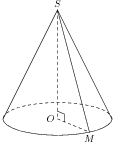
\includegraphics[scale=1]{RepS-51.png}\\ 
On va chercher à déterminer les formes géométriques permettant de
construire le patron du cône de révolution ci-contre.\\
$SM=6$~cm et $OM=4$~cm.
\end{multicols}
\begin{enumerate}
\item La base du cône est la surface engendrée par la rotation du
  segment $[OM]$ autour de l'axe $(SO)$. Quelle est la nature de cette
  base ? Construire son patron sur une feuille blanche.
\item La surface conique est la surface engendrée par la rotation du
  segment $[SM]$ autour de l'axe $(SO)$. $[SM]$ est une génératrice du
  cône.\\
Les figures ci-dessous ne sont pas à l'échelle. Parmi ces figures,
laquelle représente un patron de la surface conique du cône de
révolution ? Construire cette surface sur la même feuille que le
patron de la base et terminer le patron du cône.\\
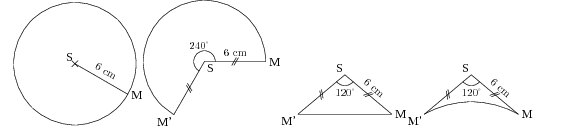
\includegraphics[scale=1]{RepS-51b.png} 
\item Quelle est la partie commune à la base et à la surface conique ?
  En déduire une égalité entre une longueur de la base et une longueur
  de la surface conique.
\end{enumerate}
\textsc{Partie B}
\begin{multicols}{2}
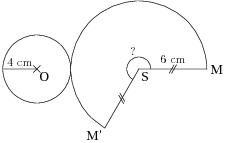
\includegraphics[scale=1]{RepS-51c.png} \\
On va chercher maintenant à déterminer pourquoi la mesure de l'angle
pour la surface conique est 240\degres. Le schéma ci-contre représente
un patron du cône de révolution étudié précédemment. On ne peut pas
construire le patron sans connaître la mesure de l'angle
$\widehat{MSM'}$.
\end{multicols}
\begin{enumerate}
\item Calculer la valeur exacte du périmètre de la base du cône.
\item 
  \begin{enumerate}
  \item Quelle est la valeur exacte de la longueur de l'arc de cercle
    $\widearc{MM'}$?
  \item Quelle serait la valeur exacte de la longueur de l'arc de
    cercle $\widearc{MM'}$ si l'angle $\widehat{MSM'}$ mesurait
    360\degres\ ?
  \end{enumerate}
\item On précise que la longueur d'un arc de cercle (ici
  $\widearc{MM'}$) est proportionnelle à la mesure de l'angle au
  centre (ici $\widehat{MSM'}$).\\
  \begin{center}
    \begin{tabular}{|l|c|c|}
      \hline
      Mesure de l'angle $\widehat{MSM'}$ (en degrés)& 360 & \phantom{216}\\
      \hline
      Longueur de l'arc de cercle $\widearc{MM'}$ (en cm) &&\\
      \hline
    \end{tabular}
  \end{center}
  Recopier et compléter le tableau ci-dessus à l'aide des questions
  précédentes et déterminer la mesure de l'angle $\widehat{MSM'}$
  permettant de construire le patron du cône.
\end{enumerate}